\documentclass{article}

\usepackage{graphicx}
\usepackage[ngerman]{babel}
\usepackage{datetime}
\usepackage{float}

\title{Projektarbeit \\ Datenbankding}
\date{08-06-2021}
\author{Severin Gafner \and David Hänni}
\newdateformat{germanformat}{\THEDAY{ }\monthname[\THEMONTH], \THEYEAR}
\def\Cmodule{Objektorientiertes Programmieren 2} 
\def\Ctitle{DatationBase} 
\def\Cauthor{Severin Gafner | David Hänni} 
\def\Cschool{TEKO Schweizerische Fachschule} 
\begin{document}

\begin{titlepage}
	\centering
	
\includegraphics[width=0.3\textwidth]{images/teko-logo-pink.jpg}\par\vspace{1cm}
	{\scshape\LARGE \Cschool\par}
	\vspace{1cm}
	{\scshape\Large Semesterarbeit \\ \Cmodule\par}
	\vspace{1.5cm}
	{\huge\bfseries \Ctitle\par}
	\vspace{2cm}
	{\Large\itshape \Cauthor\par}
	\vfill
	begleitet durch\par
	Herr Christian \textsc{Herren}

	\vfill

	{\large \germanformat\today\par}
\end{titlepage}
\pagenumbering{gobble}
\newpage
\pagenumbering{arabic}

\section{Einleitung}

Severin Gafner und David Hänni führen im Rahmen des Studiums zum Techniker HF Applikationsentwicklung für das Modul \Cmodule eine Semesterarbeit durch. 

\section{Aufgabenstellung}
Nachfolgend die Umschreibung der Aufgabenstellen 1:1 aus dem Auftrag kopiert.
\subsection{Umschreibung der Aufgabenstellung}
Wir sind die IT-Firma NewIdeas und wir haben die nachfolgende Geschäftsidee: 
Im Zusammenhang mit Automationsvorhaben werden von unseren Kunden immer mehr kleine aber individuelle Lösungen gesucht. 
Wir haben nun festgestellt, dass sich die bekannten (umfangreichen) Datenbanksysteme für derartige Vorhaben nicht oder nur bedingt eignen, vor allem die teilweise abstrus teuren Lizenzmodelle lassen diese als nur bedingt tauglich erscheinen. 
Die verfügbaren OpenSource/Freewarelösungen können wir nicht ernst nehmen resp. wollen wir aus Gründen der Nachhaltigkeit nicht verwenden.
\section{Projektumfeldanalyse}
Mit der Projekumfeldanalyse werden möglichst viele information über vorhandene Interessen, Bedürfnisse, Einflussmöglichkeiten und Beziehungen im Projektumfeld ermittelt.
\subsection{Stakeholder}
\begin{figure}[H]
	\centering
  	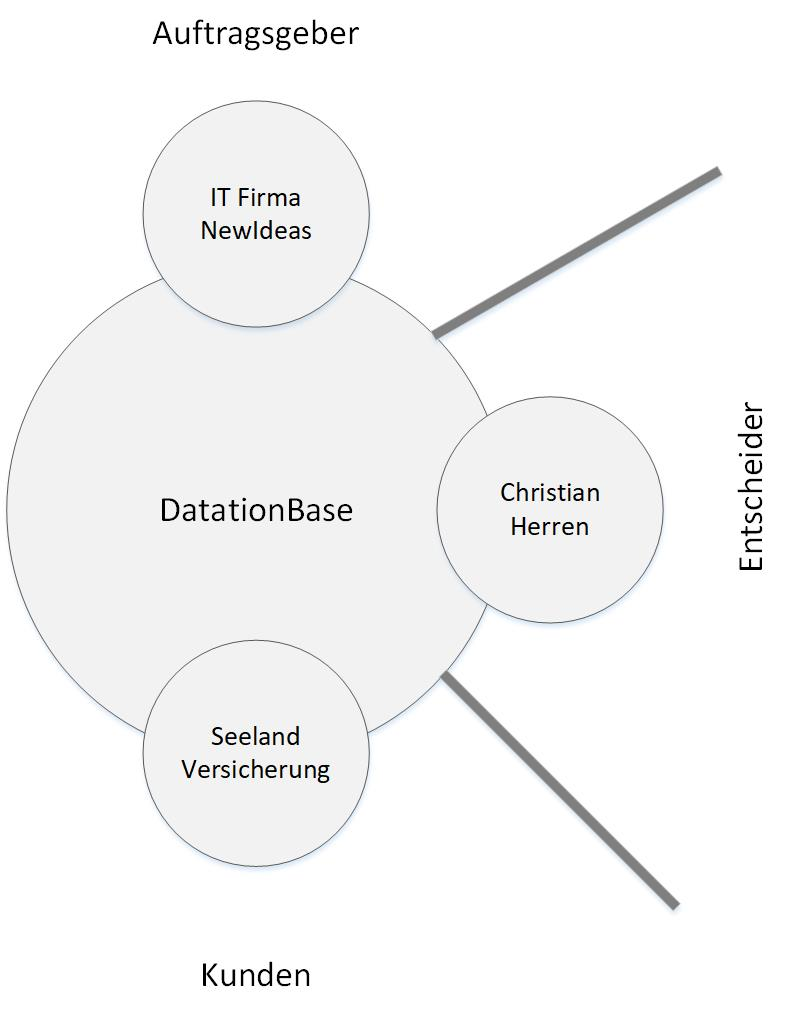
\includegraphics[width=0.7\linewidth]{images/stakeholder.jpg}
  	\caption{Identifizierte Stakeholder}
 	\label{fig:stakeholder}
\end{figure}
Die Stakeholder wurden in drei Kategorien eingeteilt:
\paragraph{Auftraggeber}
Der Auftraggeber ist die IT Firma NewIdeas. Ihr Ziel ist es, ihre Kunden mit einer eigenen Datenbanklösung an sich zu binden und so zukünftige Wartungen und Modifikationen an der Lösung durchführen zu können.
\paragraph{Kunden}
Als erstes Kunde wird die Seeland-Versicherung die Datenbank einsetzen. Später werden weitere Kunden dazustossen. Der Kunde möchte eine performante Datenbank ohne Datenverlust.
\paragraph{Entscheider}
Christoph Herren ist ebenfalls ein Stakeholder dieses Projektes. Er überwacht die Durchführung der Arbeit und bewertet das Endresultat.


\subsection{Situationsanalyse Seeland-Versicherung}
Die Seeland-Versicherung spielt als erster Kunde eine sehr wichtige Rolle. Mit den 1'500 Kunden und 450 Schadensfälle pro Jahr beinhaltet die Datenbank nur wenig Datensätze. Angenommen es werden die Schadensfälle der letzten 20 Jahre migriert, so umfasst die Datenbank immer noch nur knapp 10'000 Datensätze.
\section{Ziele}
\section{Anforderungen}
\subsection{Funktionale Anforderungen}
\subsection{Nicht funktionale Anforderungen}


\end{document}